We aimed to determine and understand the influence of risk group turnover on
the contribution of the highest risk group to the overall epidemic,
as measured by the transmission population attributable fraction (TPAF).
This section introduces a new framework for parameterizing turnover,
describes the STI model used in the experiments,
and outlines the experiments.
% ==================================================================================================
\subsection{Turnover System}
\label{ss:system}
\begin{figure}
  \centering
  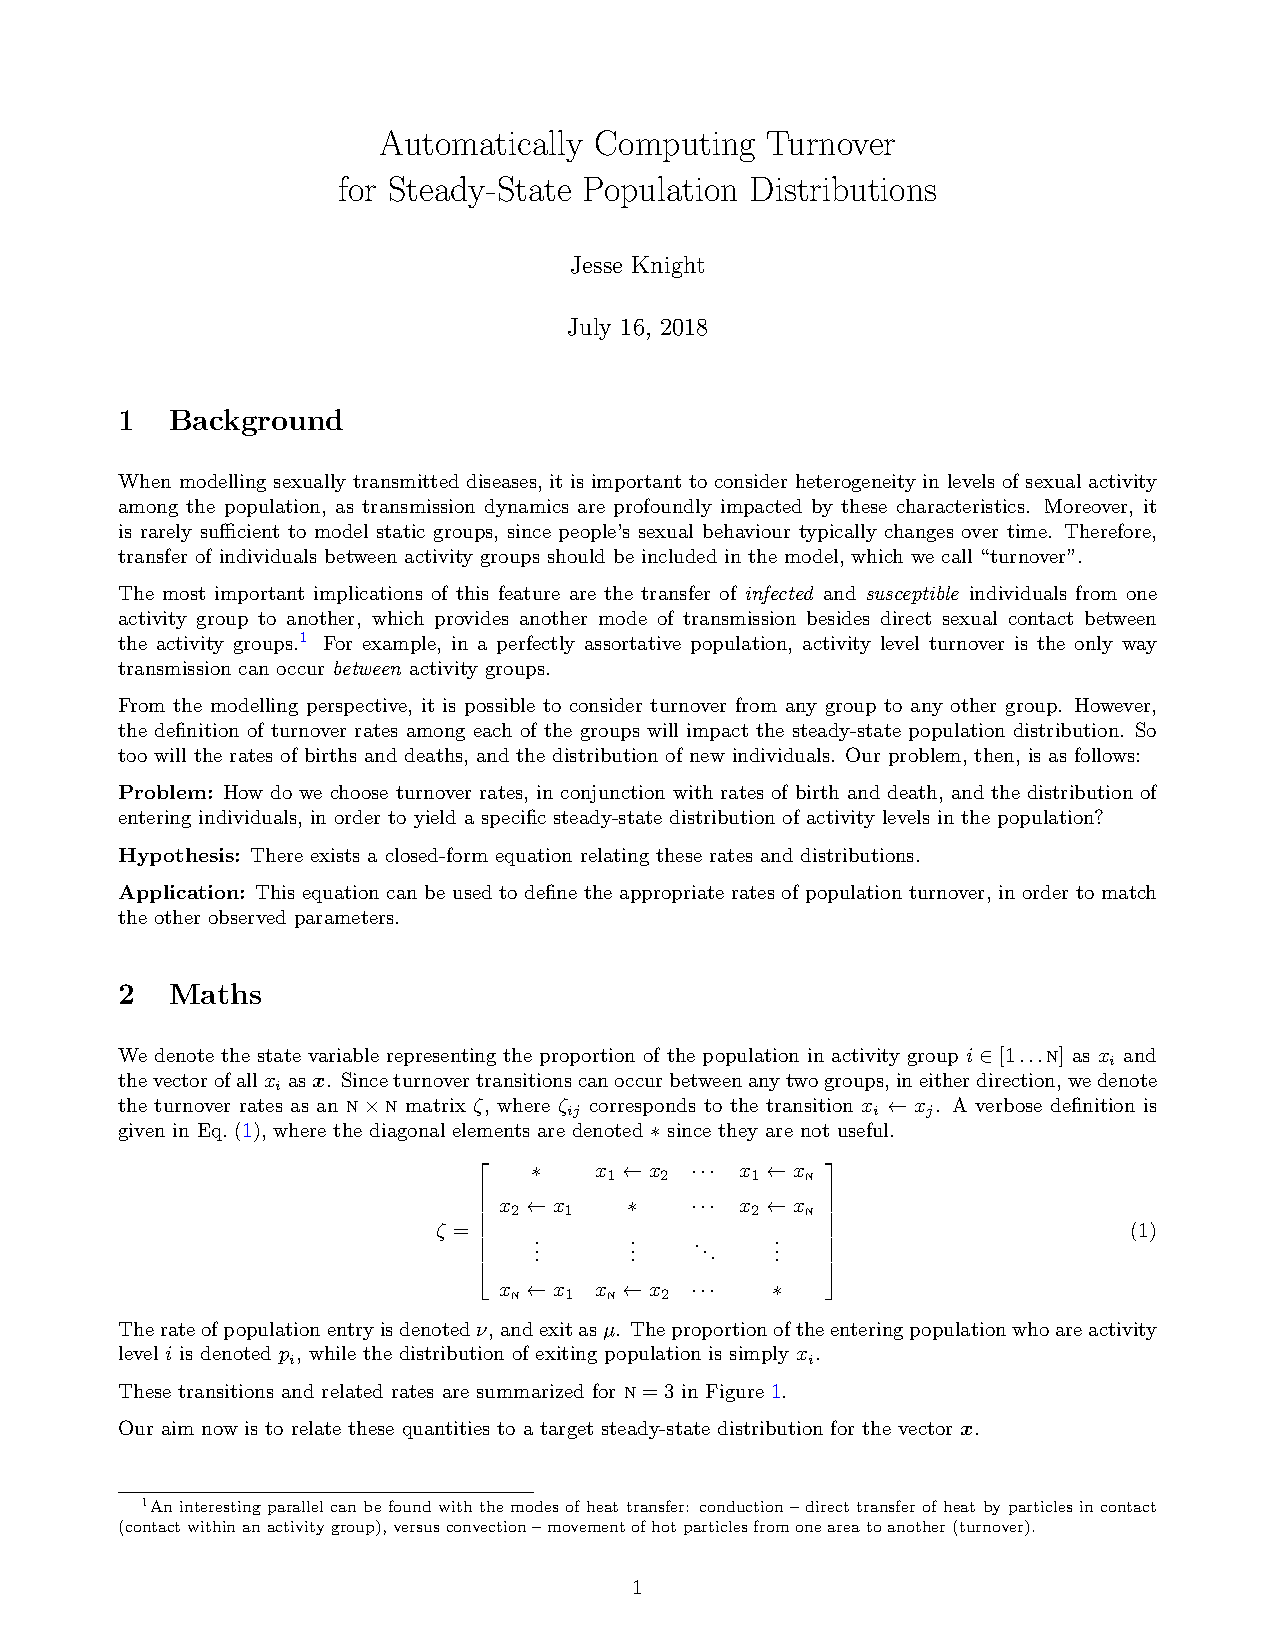
\includegraphics[width=0.5\linewidth]{turnover}
  \caption{System of risk groups and flows between them for $G = 3$}
  \label{fig:system}
\end{figure}
We developed a framework for modelling turnover,
based on the system shown in Figure~\ref{fig:system}.
A more detailed description of this framework is given in Appendix~\ref{a:system}.
The simulated population is divided into $G$ risk groups.
The number of individuals in group $i \in [1, \dots, G]$ is denoted $x_i$,
and the relative size of each group is denoted $\hat{x}_i = x_i / N$,
where $N$ is the total population size.
Individuals enter the population at a rate $\nu$ and exit at a rate $\mu$ per year.
The distribution of risk groups among individuals entering into the model
is denoted $\hat{e}_i$, which may be different from $\hat{x}_i$.
The total number of individuals entering into group $i$ per year
is therefore given by $\nu \hat{e}_i N$.
Turnover rates are collected in a $G \times G$ matrix $\phi$,
where $\phi_{ij}$ is the proportion of individuals in group $i$
who move from group $i$ into group $j$ each year.
We assume that rates of turnover $\phi$
are not affected by the health state of individuals.
\par
We assume that the relative sizes of risk groups in the model
$\bm{\hat{x}} = [\hat{x}_1, \dots, \hat{x}_G]$
are known and should remain constant over time.
We also assume that the rates of population entry $\nu$ and exit $\mu$
are known, but that they may vary over time.
Methods to estimate $\nu$ and $\mu$ are given in Appendix~\ref{aaa:params-nu-mu}.
What remains is to estimate $\bm{\hat{e}}$ and $\phi$,
representing $G + G(G-1) = G^2$ unknown values.
In the proposed framework,
these variables are collected in the vector
$\bm{\theta} = \left[\bm{\hat{e}}, \bm{y}\right]$,
where $\bm{y} = \mathrm{vec}_{i \ne j}(\phi)$.
We then construct a set of linear constraints based on data
to uniquely determine the elements of $\bm{\theta}$.
Using this approach, each constraint $k$ takes the form
$b_k = A_k \bm{\theta}$,
where $b_k$ is a constant and $A_k$ is a vector with the same length as $\bm{\theta}$.
The values of $\bm{\theta}$ can then be obtained by solving
%\begin{equation}\label{eq:system-matrix}
$\bm{\theta} = A^{-1}\bm{b}$,
%\end{equation}
for which many algorithms exist~\citep{LAPACK}.
\par
We define four types of constraints which can used to
solve for the values of $\bm{\hat{e}}$ and $\phi$ via $\bm{\theta}$.
These constraints can be selected and combined together in a flexible way,
depending on the availability of data and plausibility of assumptions.
However, a minimum of $G^2$ non-redundant constraints must be specified
to ensure a ``unique solution''
-- exactly one value of $\bm{\theta}$ which satisfies all constraints.
The four types of constraints, and the data to required to define them,
are summarized in Table~\ref{tab:constraints}.
Additional details, including
constraint equations, examples, and considerations for combining constraints,
are given in Appendix~\ref{aaa:params-turnover}.%
\begin{table}
  \centering
  \caption{Summary of constraint types for defining risk group turnover}
  \label{tab:constraints}
  \begin{tabular}{clccl}
	\toprule
	   & Name                       &            Eq.            &        E.g.         & Data requirements                                                         \\
	\midrule
	1. & Constant group size        & (\ref{eq:mass-balance-2}) & (\ref{eq:eg-basis}) & all values of $\hat{x}_i$ and $\nu$                                       \\
	2. & Specified elements         &   (\ref{eq:spec-elem})    & (\ref{eq:eg-spec})  & any value of $\hat{e}_i$ or $\phi_{ij}$                                   \\
	3. & Group duration             & (\ref{eq:duration-group}) &  (\ref{eq:eg-dur})  & any value of $\delta_i$                                                   \\
	4. & Relative rates of turnover &     (\ref{eq:ratio})      & (\ref{eq:eg-ratio}) & any relationship between two turnover rates $\phi_{ij}$ and $\phi_{i'j'}$ \\
	\bottomrule
\end{tabular}\\[1em]
\footnotesize\flushleft
$\nu$:~rate of population entry;
$\phi_{ij}$:~rate of turnover from group $i$ to group $j$;
$\hat{x}_i$:~proportion of individuals in risk group $i$;
$\hat{e}_i$:~proportion of individuals entering into risk group $i$;
$\delta_i$:~average duration spent in risk group $i$.
\end{table}
% ==================================================================================================
\subsection{Model \& Simulations}\label{ss:model-sim}
To run our experiments,
we developed a deterministic single-sex susceptible-infectious-treated (SIT) model
which simulates transmission in a population with heterogeneity in risk.
The model is not representative of a specific infection
% SS: I think it might be easier to follow if it did.
%     I think it could be used as an example to thread across
%     and then in the discussion go into how this would be similar/different for another infection
%     (which parameters would likely change,
%     whether we would anticipate that the impact of turnover would be similar, different)
% SB: I get saying any STI—but some are curative and some aren’t. ie, you can treat some
%     folks but the infection may be sustained and in others it is totally gone.
%     So just ask the question as whether we want to specify more about which type of STI
%     might be included in a model like this.
% JK: Ugh, I know, but at this point I'm not sure we can change it.
%     I really do believe that the trends in the results will hold for other STIs though.
but includes transmission via partnerships
as per sexually transmitted infections \citep{Garnett1994}.
% SB: Not sure what this means.
% JK: As to differentiate it from "mass-action" infections like the flu,
%     since we are submitting to Epidemics.
%     I've updated for clarify, hopefully
The model includes three health states:
susceptible~$\mathcal{S}$, infectious~$\mathcal{I}$, and treated~$\mathcal{T}$
(Figure~\ref{fig:health-states}),
and $G = 3$ levels of risk:
high~$H$, medium~$M$, and low~$L$.
\begin{figure}
  \centering
  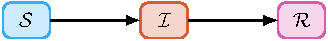
\includegraphics[width=0.4\linewidth]{health-states}
  \caption{Modelled health states.
    $\mathcal{S}$: susceptible;
    $\mathcal{I}$: infected;
    $\mathcal{T}$: treated;
    $\lambda$: force of infection;
    $\tau$: treatment.}
  \label{fig:health-states}
\end{figure}
Risk strata are defined by different number of contacts per year
so that individuals in risk group $i$ are assumed to
form contacts at a rate $C_{i}$ per year.
The probability of contact formation $\rho_{ik}$ between individuals in group $i$
and individuals in risk group $k$ is assumed to be
proportionate to the total number of available contacts within each group:
\begin{equation}
\rho_{ik} = \frac
{C_k x_k}
{\sum_{\mathrm{k}}C_{\mathrm{k}} x_{\mathrm{k}}}
\label{eq:rho}
\end{equation}
\par
The biological probability of transmission is defined as $\beta$ per contact.
Individuals transition from the
susceptible $\mathcal{S}$ to infectious $\mathcal{I}$ health-state
via a force of infection $\lambda$ per year, per susceptible in risk group $i$:
\begin{equation}
\lambda_{i} =
C_{i} \sum_k \rho_{ik} \thinspace  \beta \thinspace \frac{\mathcal{I}_k}{x_k}
\label{eq:foi}
\end{equation}
Individuals are assumed to transition from the
infectious $\mathcal{I}$ to treated $\mathcal{T}$ health-state
at a rate $\tau$ per year, reflecting diagnosis and treatment.
The treatment rate is not stratified by risk group.
Individuals in the treated $\mathcal{T}$ health-state are not infectious nor susceptible,
and individuals cannot become re-infected.
% SS: What seems confusing to me at this point is that
%     given the lack of specificity of the infection of interest,
%     the R assumptions seem potentially overly simplistic
%     given that with most STIs there is unlikely to be immunity following recovery
%     and in the case of HIV, treatment (if considered R) may be stopped/incomplete
%     and then they may not be susceptible, but certainly transmittable.
% JK: I guess I could try to justify this by saying that
%     allowing R -> I transitions (coming off treatment)
%     could be approximated by a slower I -> R (treatment) rate,
%     since it would result in more people in I than R.
%     So, I don't think the results would change too much
% --------------------------------------------------------------------------------------------------
\subsubsection{Turnover implementation}
As described in Section~\ref{ss:system}, individuals
enter the model at a rate $\nu$,
exit the model at a rate $\mu$,
and transition from risk group $i$ to group $j$ at a rate $\phi_{ij}$.
The turnover rates $\phi$ and
distribution of individuals entering the model by risk group $\bm{\hat{e}}$
were computed using the methods outlined in
Appendix~\ref{aaa:params-turnover}, based on the following assumptions.
% SB: Do we need to explain why we made these assumptions? Or provide refs?
% JK: Since we are constructing a simulated system, I'm not sure what refs might be appropriate,
%     but, you make a great point about justifying.
%     I've added a sentence after all 3 assumptions explaining.
%     I think I was avoiding this because it was hard to explain,
%     but let me know how it reads.
First, we assumed that
the proportion of individuals entering each risk group $\bm{\hat{e}}$
was equal to the proportion of individuals across risk groups in the model $\bm{\hat{x}}$.
% LW: And another strong assumption which was implicit here is that u assume
%     the rate of turn over to be the same irrespective of disease status.
%     And I think it is critical to make it explicit.
%     So S, I, T all have the same turn over rate,
% JK: So, I did now include this in the Turnover System section (last sentence).
%     Do you think it needs to be restated here?
Second, we assumed that
the average duration spent in each risk group $\bm{\delta}$ is known.
Third, we assumed that
the absolute number of individuals moving between two risk groups in either direction is balanced.
% LW: I would think this is a very strong assumption.
%     It is essentially saying the turn-over system consistently
%     *swap* individuals in two risk groups.
% HM: Not fully understand how does this assumption work?
%     If high risk group has 10 individuals move to medium group,
%     medium group will move 10 individuals to high risk? This is independent from population entry?
% JK: @HM: yes, this is what this assumption means. I've edited hopefully to be more clear.
%     @LW: see new sentence below. We have to make at least one more assumption,
%     else the system will not have a unique solution,
%     and by "balancing" the turnover rates, it is a way of avoiding "bias":
These assumptions were chosen to avoid any dominant direction of turnover,
so that the effects of turnover on model outputs would be
attributable to movement of people between risk groups in general,
rather than in one specific direction.
The system of equations which results from these assumptions
is given in Appendix~\ref{aa:eqs-turnover}.
To meet all three conditions, there is only one possible value
for each element in $\phi$ and $\bm{\hat{e}}$.
In other words, by specifying these three conditions,
we ensure that a unique set of $\phi$ and $\bm{\hat{e}}$ is computed.
\par
Using the above three assumptions,
we need to specify the values of $\bm{\hat{x}}$, $\bm{\delta}$, $\nu$, and $\mu$.
Such parameters could be derived from data as described in Section~\ref{aaa:params-turnover};
however, in this experiment, we use the illustrative values summarized in
Table~\ref{tab:params}.
% LW: After read the whole results section,
%     I think experiment 2 and 3.2 followed values specified in Table 3.
%     But experiment 1 and 3.1 explored a wide range of
%     turn-over and treatment rates.
%     it is unclear what do u refer to when u said “this experiment”.
%     Given the organization and length – by the time I reached results of Experiemnt 2,
%     I almost forgot under which values they were done – as the section preceed it
%     explored a range of values of turn-over rate and treatment rate.
% JK: Hopefully now with the paper much much shorter, this is resolved?
After resolving the system of equations,
$\bm{\hat{e}}$ is equal to $\bm{\hat{x}}$ (assumed), and $\phi$ is:
\begin{equation}
\label{eq:phi-values}
\phi = \left[\begin{array}{ccc}
* & 0.0833 & 0.0867\\
0.0208 & * & 0.0158\\
0.0058 & 0.0042 & *
\end{array}\right]

\end{equation}
\begin{table}
  \centering
  \caption{Model parameters}
  \label{tab:params}
  \begin{tabular}{clc}
	\toprule
	    Symbol     & Description                                                     &            Value             \\
	\midrule
	 $\bm{\beta}$  & transmission probability per contact                            &            $0.03$            \\
	    $\tau$     & rate of treatment initiation among infected                     &            $0.1$             \\
	    $N_0$      & initial population size                                         &            $1000$            \\
	\midrule
	$\bm{\hat{x}}$ & proportion of system individuals by risk group                  & $[ 0.05 \es 0.20 \es 0.75 ]$ \\
	$\bm{\hat{e}}$ & proportion of entering individuals risk by risk group           & $[ 0.05 \es 0.20 \es 0.75 ]$ \\
	$\bm{\delta}$  & average duration spent in each risk group                       &    $[ 5 \es 15 \es 25 ]$     \\
	     $C$       & rate of contact formation among individuals in each risk group  &     $[ 25 \es 5 \es 1 ]$     \\
	    $\nu$      & rate of population entry                                        &            $0.05$            \\
	    $\mu$      & rate of population exit                                         &            $0.03$            \\
	\bottomrule
\end{tabular}
  % SS: All of this seems a little hard to follow in terms of the infection,
  %     b/c it seems to indicate that there is an underlying infection of interest,
  %     but it is not being stated.
  % JK: Same as above, not sure what to say here...
  %     We did start out with HIV, but since we're not considering STI-mortality,
  %     we really cannoy call it HIV.
\end{table}
\par
We then simulated epidemics using these parameters.
The model was initialized with $N_0 = 1000$ individuals
who are distributed across risk groups according to $\bm{\hat{x}}$.
We seeded the epidemic with
one infectious individual in each risk group at $t = 0$.
There were no treated individuals at the start of the epidemic,
and so all individuals except the 3 infectious individuals were susceptible.
We numerically solved the system of ordinary differential equations
in Python%
\footnote{Code for all aspects of the project is available at:
  \href{https://github.com/c-uhs/turnover}{\texttt{https://github.com/c-uhs/turnover}}}
using Euler's method with a time step of $dt = 0.1$ years.
The full system of model equations is given in Appendix~\ref{aa:eqs-model}.
All comparative analyses are then conducted at equilibrium,
defined as a steady state at 500 years with $<1\%$ difference in incidence per year.
% ==================================================================================================
\subsection{Experiments}
\label{ss:exp}
The experiments used to examine
the influence of risk group turnover on model outputs
are as follows.
% --------------------------------------------------------------------------------------------------
\subsubsection{Experiment~1: Influence of turnover on equilibrium incidence and prevalence}
\label{sss:exp-prev-inc}
Experiment~1 examined the influence of turnover on
equilibrium incidence and prevalence, across each risk group and overall.
Incidence was defined as $\lambda_i$ from Eq.~(\ref{eq:foi}), and
prevalence was defined as $\hat{\mathcal{I}}_i = \dfrac{\mathcal{I}_i}{\mathcal{X}_i}$.
% SM: start by something like this to orient the reader
%     and help with interpretation before results section
% JK: I agree this could be useful, but then we go back-and forth between
%     implementation ("controlled by a single parameter") and
%     an overview of the experiment ("influence of turnover on ...")
%     I'd rather introduce how turnover is controlled via duration in high risk group
%     after noting why we cannot simply scale the rates proportionally with a single parameter.
As in similar experiments \citep{Zhang2012,Henry2015},
the rates of turnover were scaled by a single parameter.
However, because the model had $G = 3$ risk groups,
multiplying a set of base rates $\phi$ by a scalar factor
would have resulted in changes to the relative population size of risk groups $\bm{\hat{x}}$.
Thus, we controlled the rates of turnover using
the duration of individuals in the high risk group $\delta_H$,
such that a shorter $\delta_H$ implied higher rates of turnover among all groups.
The duration of individuals in the medium risk group $\delta_M$
was then defined as a value between $\delta_H$ and the maximum duration $\mu^{-1}$
which scaled with $\delta_H$ following:
$\delta_M = \delta_H + \kappa \left(\mu^{-1} - \delta_H\right)$, with $\kappa = 0.3$.
The duration of individuals in the low risk group $\delta_L$
similarly scaled with $\delta_H$,
but due to existing constraints,
specification of $\delta_H$ and $\delta_M$
results in only one possible value of $\delta_L$.
In this way, each value of $\delta_H$ was used to define a unique set of turnover rates $\phi$
whose elements all scaled inversely with the duration in the high risk group $\delta_H$.
The value of $\delta_H$ was then varied from 33~to~3 years
to examine the influence of different turnover rates.
The resulting durations in each group are shown in Figure~\ref{fig:dur-group}.
\begin{figure}
  \centering\includegraphics[width=0.45\linewidth]{{1d-dur-all-tau=0.1}.pdf}
  \caption{Average duration in each risk group as turnover rates vary.}
  \label{fig:dur-group}
\end{figure}
\par
We plotted the STI prevalence versus turnover for each risk group,
and explored mechanisms which explained the observed trends,
including movement of individuals between risk groups, and incidence.
We also plotted the STI prevalence ratios between each combination of risk groups,
to help form a basis for understanding the results of Experiments~2~and~3.
% --------------------------------------------------------------------------------------------------
\subsubsection{Experiment~2: Inferred risk heterogeneity with vs without turnover}
\label{sss:exp-infer}
Next, we examined the influence of turnover on
the parameter values inferred via model fitting.
Specifically, we fit the model, with and without turnover, to:
20\% infection prevalence among the high risk group,
8.75\% among the medium risk group,
3\% among the low risk group,
and 5\% overall.
We fit the contact rates $C$ of all risk groups
by minimizing the negative log-likelihood of each predicted prevalence versus the target.%
\footnote{Sample sizes of 500, 2000, 7500, and 10,000 were assumed to generate binomial distributions
  for the high, medium, low, and overall prevalence targets respectively,
  and the minimization was performed using
  the SLSQP method~\citep{Kraft1988} from the SciPy Python package
  (\href{https://docs.scipy.org/doc/scipy/reference/generated/scipy.optimize.minimize.html}
  {\texttt{scipy.optimize.minimize}}).}
We then compared the inferred contact rates $C$
in the model with versus without turnover.
The ratio of fitted (or posterior) contact rates $C_H~/~C_L$
represents a measure of risk heterogeneity in the population,
after fixing all other parameters,
which produces the given infection prevalence.
% --------------------------------------------------------------------------------------------------
\subsubsection{Experiment~3: Influence of turnover on the TPAF of the highest risk group}
\label{sss:exp-tpaf}
Finally, Experiment~3 examined how
the estimated contribution of highest risk group to overall transmission,
as measured by the transmission population attributable fraction (TPAF),
varied with versus without turnover.
The TPAF of a risk group $i$ is defined as:
\begin{equation}
\textsc{tpaf}_i(t) = \frac{I_0(t) - I_i(t)}{I_0(t)}
\end{equation}
where $I_0(t)$ is the cumulative number of new infections
by time $t$ under usual conditions,
and $I_i(t)$ is the cumulative number of new infections
assuming no transmission from risk group $i$.
Both $I_0(t)$ and $I_i(t)$ are calculated
starting from a system at equilibrium.
\par
We compared the two fitted models from Experiment~2,
which were identical in structure except that
one model had no turnover and one model had turnover
(default parameterization described in Section~\ref{ss:model-sim}).
While prevalence was the same in both models,
the group-specific contact rates inferred via model fitting were different.
Following equilibration of both models,
the TPAF of the high risk group was then estimated over a continuous time horizon.
